\documentclass[]{elsarticle} %review=doublespace preprint=single 5p=2 column
%%% Begin My package additions %%%%%%%%%%%%%%%%%%%

\usepackage[hyphens]{url}

  \journal{SoftwareX} % Sets Journal name

\usepackage{lineno} % add
  \linenumbers % turns line numbering on

\usepackage{graphicx}
%%%%%%%%%%%%%%%% end my additions to header

\usepackage[T1]{fontenc}
\usepackage{lmodern}
\usepackage{amssymb,amsmath}
\usepackage{ifxetex,ifluatex}
\usepackage{fixltx2e} % provides \textsubscript
% use upquote if available, for straight quotes in verbatim environments
\IfFileExists{upquote.sty}{\usepackage{upquote}}{}
\ifnum 0\ifxetex 1\fi\ifluatex 1\fi=0 % if pdftex
  \usepackage[utf8]{inputenc}
\else % if luatex or xelatex
  \usepackage{fontspec}
  \ifxetex
    \usepackage{xltxtra,xunicode}
  \fi
  \defaultfontfeatures{Mapping=tex-text,Scale=MatchLowercase}
  \newcommand{\euro}{€}
\fi
% use microtype if available
\IfFileExists{microtype.sty}{\usepackage{microtype}}{}
\usepackage[]{natbib}
\bibliographystyle{plainnat}

\ifxetex
  \usepackage[setpagesize=false, % page size defined by xetex
              unicode=false, % unicode breaks when used with xetex
              xetex]{hyperref}
\else
  \usepackage[unicode=true]{hyperref}
\fi
\hypersetup{breaklinks=true,
            bookmarks=true,
            pdfauthor={},
            pdftitle={Microxanox - an R package for simulating an MICRobial ecosystem that can occupy OXic or ANOXic states.},
            colorlinks=true,
            urlcolor=blue,
            linkcolor=blue,
            pdfborder={0 0 0}}

\setcounter{secnumdepth}{5}
% Pandoc toggle for numbering sections (defaults to be off)


% tightlist command for lists without linebreak
\providecommand{\tightlist}{%
  \setlength{\itemsep}{0pt}\setlength{\parskip}{0pt}}

% From pandoc table feature
\usepackage{longtable,booktabs,array}
\usepackage{calc} % for calculating minipage widths
% Correct order of tables after \paragraph or \subparagraph
\usepackage{etoolbox}
\makeatletter
\patchcmd\longtable{\par}{\if@noskipsec\mbox{}\fi\par}{}{}
\makeatother
% Allow footnotes in longtable head/foot
\IfFileExists{footnotehyper.sty}{\usepackage{footnotehyper}}{\usepackage{footnote}}
\makesavenoteenv{longtable}


%% \documentclass[preprint,12pt, a4paper]{elsarticle}

%% Use the option review to obtain double line spacing
%% \documentclass[authoryear,preprint,review,12pt]{elsarticle}

%% For including figures, graphicx.sty has been loaded in
%% elsarticle.cls. If you prefer to use the old commands
%% please give \usepackage{epsfig}

%% The amssymb package provides various useful mathematical symbols
\usepackage{amssymb}
%% The amsthm package provides extended theorem environments
%% \usepackage{amsthm}

%% The lineno packages adds line numbers. Start line numbering with
%% \begin{linenumbers}, end it with \end{linenumbers}. Or switch it on
%% for the whole article with \linenumbers.
\usepackage{lineno}

\usepackage{float}
\restylefloat{table}

\journal{SoftwareX}

%\usepackage{lineno}
%\linenumbers
%\usepackage{setspace}
%\doublespacing
%\usepackage{fancyhdr}
%\fancyhead{}
%\fancyfoot{}
%\fancyhead[CO,CE]{Microxanox R package}
%\pagestyle{fancy}
%



\begin{document}


\begin{frontmatter}

  \title{Microxanox - an R package for simulating an \(MICR\)obial
ecosystem that can occupy \(OX\)ic or \(ANOX\)ic states.}
    \author[University of Zürich]{Rainer M Krug%
  %
  \fnref{Corresponding Author}}
   \ead{Rainer.Krug@uzh.ch; Rainer@krugs.de} 
    \author[University of Zürich]{Owen L. Petchey}
   \ead{Owen.Petchey@ieu.uzh.ch} 
      \affiliation[University of Zürich]{Department of Evolutionary
Biology and Environmental Studies, Winterthurerstrasse 190, 8057 Zurich}
    \cortext[cor1]{Corresponding author}
    \fntext[1]{Corresponding Author}
    \fntext[2]{Equal contribution}
  
  \begin{abstract}
  Ca. 100 words.
  \end{abstract}
    \begin{keyword}
    metadata quality; data curation; archival; long term storage; R
package; \sep 
    metadata quality; data curation; archival; long term storage; R
package;
  \end{keyword}
  
 \end{frontmatter}

\hypertarget{todo}{%
\section{\texorpdfstring{\color{red}TODO}{TODO}}\label{todo}}

\begin{itemize}
\tightlist
\item
  \color{red}\textbf{update links}
\item
  \color{red}\textbf{update cross references} \pagebreak
\end{itemize}

\hypertarget{required-metadata}{%
\section{Required Metadata}\label{required-metadata}}

\hypertarget{current-code-version}{%
\subsection{Current code version}\label{current-code-version}}

Ancillary data table required for subversion of the codebase.

\begin{longtable}[]{@{}
  >{\centering\arraybackslash}p{(\columnwidth - 4\tabcolsep) * \real{0.0596}}
  >{\raggedright\arraybackslash}p{(\columnwidth - 4\tabcolsep) * \real{0.4106}}
  >{\raggedright\arraybackslash}p{(\columnwidth - 4\tabcolsep) * \real{0.5298}}@{}}
\toprule
\begin{minipage}[b]{\linewidth}\centering
\textbf{Nr.}
\end{minipage} & \begin{minipage}[b]{\linewidth}\raggedright
\textbf{Code metadata description}
\end{minipage} & \begin{minipage}[b]{\linewidth}\raggedright
\textbf{Please fill in this column}
\end{minipage} \\
\midrule
\endhead
C1 & Current code version & v0.9.0 \\
C2 & Permanent link to code/repository used for this code version &
\url{https://github.com/UZH-PEG/microxanox} \\
C3 & Code Ocean compute capsule & \\
C4 & Legal Code License & CC BY 4.0 \\
C5 & Code versioning system used & git \\
C6 & Software code languages, tools, and services used & R \\
C7 & Compilation requirements, operating environments & R (\textgreater=
4.1.0), ADD PACKAGES \\
C8 & If available Link to developer documentation/manual & \\
C9 & Support email for questions & Rainer.Krug@uzh.ch;
Rainer@krugs.de \\
\bottomrule
\end{longtable}

\hypertarget{motivation-and-significance}{%
\section{Motivation and
significance}\label{motivation-and-significance}}

Many ecosystems are exposed to gradual changes of environmental
variables, to which the responses are not always as gradual as the
change of the environmental variable. One example where the gradual
change of a single environmental variable is causing an abrupt change of
the system is the switch from an aerobic to anaerobic system. This
system has been investigated by \citet{Bush2017}. We wanted to take this
investigation one step further, and look at the role an increased
biodiversity plays in these dynamics \citep{REF_NEEDED}. For this
purpose, we developed this package.

The microxanox package is a package for simulating a three functional
group system (\emph{CB}: cyanobacteria, \emph{PB}: phototrophic sulfur
bacteria, and \emph{SB}: sulfate-reducing bacteria) with four chemical
substrates (\emph{P}: phosphorus, \emph{O}: oxygen, \emph{SR}: reduced
sulfur, \emph{SO}: oxidized sulfur). It includes feedback between
biogeochemical processes and is based on \citep{Bush2017} (See
\citep{Bush2017} for a detailed discussion of the model).

The aims of the \texttt{microxanox} package are twofold. Firstly, the
package aims at reproducing the results shown by \citep{Bush2017}, which
is accomplished in the \href{LINK\%20NEEDED}{vignette Partial
reproduction of Bush et al}. Secondly, to take these results one step
further, it includes new functionality to address our research question
as published in \citep{REF_NEEDED}.

For this, we extended the model and added functionality for:

\begin{itemize}
\tightlist
\item
  Multiple strains (effectively unlimited) per functional group.
\item
  Adding temporally varying oxygen diffusivity.
\item
  Adding random noise in substrate concentrations.
\item
  Including immigration.
\item
  Setting minimum population abundances.
\end{itemize}

In addition to the model itself, the package includes some functions to
analyse the results as well as visualize the results to provide a
starting point for customized visualizations based on own requirements.

\hypertarget{software-description}{%
\section{Software description}\label{software-description}}

\begin{quote}
\{\textgreater\textgreater Describe the software in as much as is
necessary to establish a vocabulary needed to explain its
impact.\textless\textless\}
\end{quote}

We will discuss the general structure and functionality of the package
here without going into to much detail. A more detailed discussion can
be found in the \href{LINK_NEEDED}{User Guide}.

The model by \citet{Bush2017} is based on ODEs for the rates of change
which are specified in the function \texttt{bushplus\_dynamic\_model()}.
This augmented version of the model published in \citep{Bush2017} can
handle multiple strains within each of the three functional groups,
temporal variation in oxygen diffusivity, and events.

The package is not intended to provide a modelling framework which can
be adjusted easily to all needs, but primarily a tool to implement the
model used by \citep{Bush2017} and to extend it to our needs
\citep{REF_NEEDED}. Consequently, any more substantial changes and
adaptations are likely to need a change in the source code.

Nevertheless, the source code is structured in modular, so that e.g.~the
event definition can easily be changed, or other aspects can be
adjusted. All values in the parameter object can be changed as needed
and the general structure of the code should make it not to difficult to
adapt the model to other similar systems.

\hypertarget{software-architecture}{%
\subsection{Software Architecture}\label{software-architecture}}

\begin{quote}
\{\textgreater\textgreater Give a short overview of the overall software
architecture; provide a pictorial component overview or similar (if
possible). If necessary provide im- plementation
details.\textless\textless\}
\end{quote}

The framework used when writing this package aims at reproducibility of
the results. It builds on the following main considerations:

\begin{enumerate}
\def\labelenumi{\arabic{enumi}.}
\tightlist
\item
  all parameter needed to run a simulation or find a stable state are
  contained in a single parameter object. This object is created by
  using the functions \texttt{new\_...\_parameter()},
  \texttt{new\_initial\_state()} and \texttt{new\_strain\_parameter()}.
  Which one of the \texttt{new\_...\_parameter()} functions has to be
  used when, will be discussed in the section @ref(runsim) and in more
  detail in the \href{LINK_NEEDED}{User Guide}.
\item
  The function call \texttt{run\_...(parameter)} will run the simulation
  using the parameter as defined in the object \texttt{parameter}.
\item
  The return value of the \texttt{run\_...(parameter)} function is
  identical to the parameter object plus an additional slot named
  \texttt{results} which contains the results of the run
\item
  As the return value contains all parameter, it is possible to re-run
  the simulation by simply running \texttt{run\_...(result)}.
\end{enumerate}

The point that the results object contains all parameter needed to run
the simulation, promotes reproducibility and makes incremental changes
of individual parameters and re-running the simulations much easier.

In the following sections we describe the general usage of the package:
running one simulation, finding steady states across an environmental
gradient, calculating measures of stability, and visualization.

\hypertarget{running-one-simulation}{%
\subsubsection{Running one simulation}\label{running-one-simulation}}

A typical simulation would look as shown in @ref(fig:runsim\_example).

\begin{verbatim}
#> [1] "./figures/simflow.pdf"
\end{verbatim}

\begin{figure}

{\centering 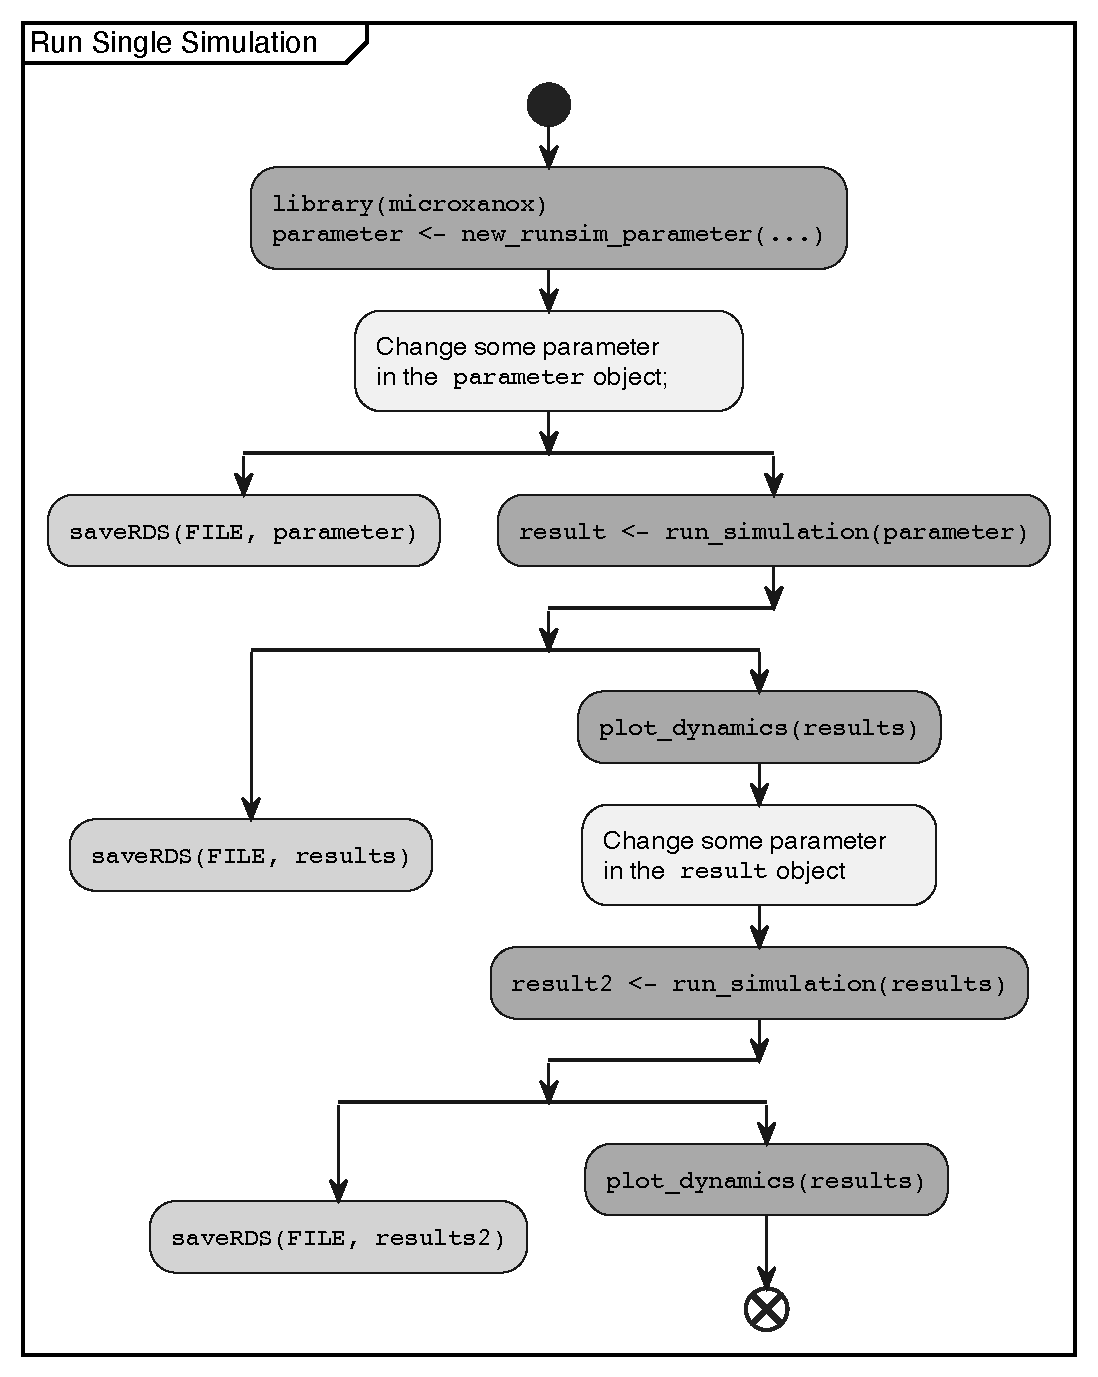
\includegraphics[width=350px]{./figures/simflow} 

}

\caption{Typical flow of a simulation. Dark Grey boxes: commands necessary for simulation; Light Grey:Saving of parameter and results; Lightest Grey: Different non specified commands.}\label{fig:runsim_example}
\end{figure}

The individual simulation (\texttt{run\_simulation()} function) is the
working horse in this package. In this function, the ODEs are solved.
The function needs only one argument - an object as created by the
function \texttt{new\_runsim\_parameter()}. One parameter of this object
is the \texttt{strain\_parameter} which can be created by the function
\texttt{new\_strain\_parameter()}. For a detailed description of the
parameter, their meaning and how they are created please see the User
Guide which accompanies the package or is available at
\href{@LINK_NEEDED}{User Guide}

After the parameter object has been defined, it can be used in the
\texttt{run\_simulation()} function. The function returns an object
which is identical to the parameter, except of an additional slot
containing the results. This design produces a fully reproducible object
as it can be used instead of a parameter object to be fed back into the
\texttt{run\_simulation()} function to run the simulation again from the
parameter used to generate the results from.

The function \texttt{plot\_dynamics()} plots a single simulation run, as
returned from the \texttt{run\_simulation()} function. This function is
only provided as a convenience function to provide a way to easily see
the results of a simulation run. An example plot resulting from this
function is shown in @ref(fig:plot-dynamics).

\begin{figure}

{\centering 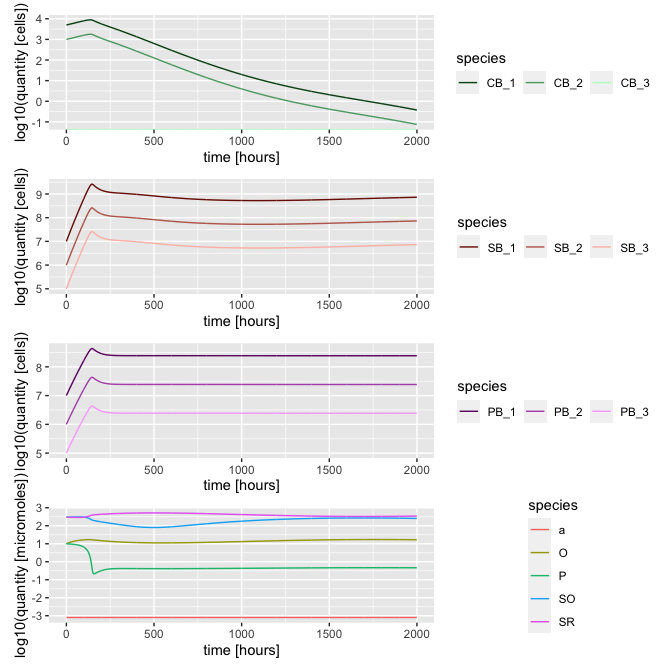
\includegraphics[width=350px]{figures/ug_three_strains_dynamics} 

}

\caption{Plot of results of a simulation run using the function $plot_dynamics()$. Details can be found in the "User Guide" section "Three strains per functional group".}\label{fig:plot-dynamics}
\end{figure}

\hypertarget{finding-a-steady-state-of-the-model}{%
\subsubsection{Finding a Steady State of the
model}\label{finding-a-steady-state-of-the-model}}

There are two methods for finding steady states. The first runs a
separate simulation for each combination of starting conditions and
oxygen diffusivity (let us term this the \emph{Replication method}). The
second runs only two simulations, with step-wise and slowly temporally
increasing or decreasing oxygen diffusivities and recorded of state just
before change to a new oxygen diffusivity (let us term this the
\emph{Temporal method}).

\hypertarget{replication-method}{%
\paragraph{Replication Method}\label{replication-method}}

The replication method is implementad in the function
\texttt{run\_replication\_ssfind()} which takes a parameter object as
returned by the function \texttt{new\_replication\_ssfind\_parameter()}
and the number of cores for multithreading the simulation.

\hypertarget{temporal-method}{%
\paragraph{Temporal Method}\label{temporal-method}}

The temporal method involves two simulations for a particular system
configuration (parameter set). In one simulation the oxygen diffusivity
is \emph{increased} in a step-wise fashion. In the other it is
\emph{decreased} in a step-wise fashion. That is, oxygen diffusivity is
held at a constant level for long enough for steady state to be reach,
that state is recorded, and then a slightly higher (or lower) oxygen
diffusivity value is set. Hence, at that time point, the system is
effectively started with initial conditions that are the state of the
system in the previous time step.

This is implemented in the function \texttt{run\_temporal\_ssfind()},
which takes a parameter object as created by the function
\texttt{new\_temporal\_ssfind\_parameter()}.

For a more detailed walk-through of these two approaches and explanation
please see the \href{@LINK_NEEDED}{User Guide}.

\hypertarget{extracting-stability-measures}{%
\subsubsection{Extracting Stability
Measures}\label{extracting-stability-measures}}

From the raw results returned by these \texttt{run\_...()} functions,
the stability measures can be extracted by using the function
\texttt{get\_stability\_measures()}. These measures include
non-linearity and hysteresis measures, of the response of the simulated
system to environmental change.

\hypertarget{use-cases}{%
\subsection{Use Cases}\label{use-cases}}

We will now show two use cases which illustrate applications of the
package. All use cases can be used as starting points for other
investigations of the behavior of the system.

The first two use cases are described in detail in the User Guide and
the Partial Reproduction Vignettes. The third is taken from
\citet{REF_NEEDED} for which this R package was designed. All of these
use cases can be expanded to larger numbers of strains per functional
group and variable values van be changed.

\hypertarget{regime-shifts-during-temporal-environmental-change}{%
\subsubsection{Regime shifts during temporal environmental
change}\label{regime-shifts-during-temporal-environmental-change}}

In the \href{LINK_NEEDED}{User Guide} we used a one strain system
(section ``1 strain per functional group'') and three strain system
(section ``3 strains per functional group'') to determine as an example
the stable states during temporal environmental changes (the oxygen
diffusivity). From these simulatiuons, we extracted measures of
nonlinearity and hysteresis. See Fig @ref(fig:plot-dynamics) as an
example plot of the simulations.

\begin{figure}

{\centering 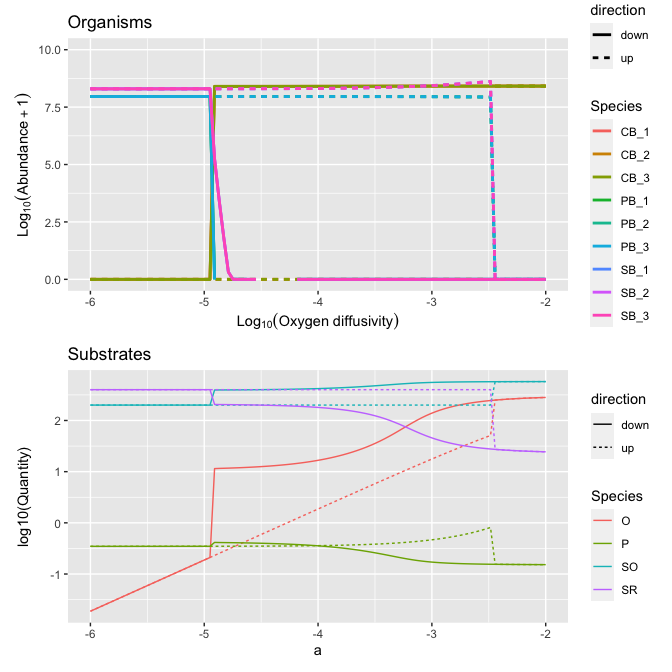
\includegraphics[width=350px]{figures/ug_three_strains_stable_state} 

}

\caption{Plot of the stable states of the simulation runs under different oxygen diffusivity. The top graph are the Organisms (ech initially with three strains) while the lower graph is the substrate availability under the same oxygen diffusivities. Details can be found in the "User Guide" section "Three strains per functional group".}\label{fig:uc1_stable_state}
\end{figure}

We saved all parameter and result objects, so that all results are
completely reproducible. The general flow of the experiment is identical
to the one shown in @ref(fig:runsim\_example).

\hypertarget{the-extent-of-hysteresis-depends-on-community-composition}{%
\subsubsection{The extent of hysteresis depends on community
composition}\label{the-extent-of-hysteresis-depends-on-community-composition}}

One of the reasons to develop this package was to reproduce the results
presented in \citet{Bush2017}. This was achieved as demonstrated in the
\href{LINK_NEEDED}{Partial Reproduction supplement}. All aspects in the
paper could be reproduced and are shown in the vignette.

\begin{figure}

{\centering 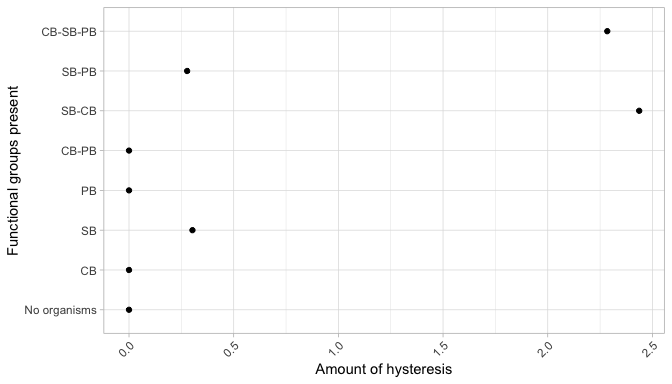
\includegraphics[width=350px]{figures/user_guide_hysteresis} 

}

\caption{Hysteresis of all assessed combinations of variability.}\label{fig:user_guide_hysteresis}
\end{figure}

Ass all objects were saved, results can be easily reproduced and
parameter can be changed to assess the impact of these changes (e.g.~to
conduc a sensitivity analysis).

\hypertarget{effects-of-functional-diversity-on-regime-shifts}{%
\subsubsection{Effects of functional diversity on regime
shifts}\label{effects-of-functional-diversity-on-regime-shifts}}

As discussed in the paper \citep{REF_NEEDED}, the role biodiversity
plays in abrupt regime shifts based on gradual changing environmental
parameter is not well understood. This model (as part of the package)
has been used to investigate these dynamics and the results are
available in \citet{REF_NEEDED}.

{\{\textgreater\textgreater More details from the
paper.\textless\textless\} \{\textgreater\textgreater Romana will
provide two or three sentences\textless\textless\}}

\hypertarget{impact}{%
\section{Impact}\label{impact}}

\begin{quote}
\{\textgreater\textgreater This is the main section of the article and
the reviewers weight the description here appropriately Indicate in what
way new research questions can be pursued as a result of the software
(if any). Indicate in what way, and to what extent, the pursuit of
existing research questions is improved (if so). Indicate in what way
the software has changed the daily practice of its users (if so).
Indicate how widespread the use of the software is within and outside
the intended user group. Indicate in what way the software is used in
commercial settings and/or how it led to the creation of spin-off
companies (if so).\textless\textless\}
\end{quote}

The free and open source implementation and extension of the model used
in \citet{Bush2017} provides the means of reproducing the results
published while at the same time provides the means of doing
investigations which extend the original publication, as done in
\citet{REF_NEEDED}.

The combination of all parameter in a single parameter object as well as
the return of the simulation as a result object which inherits from the
parameter object and adds a results slot provides a relatively easy to
use framework to implement reproducible experiments.

\hypertarget{conclusions}{%
\section{Conclusions}\label{conclusions}}

Set out the conclusion of this original software publication.

\hypertarget{conflict-of-interest}{%
\section{Conflict of Interest}\label{conflict-of-interest}}

We wish to confirm that there are no known conflicts of interest
associated with this publication and there has been no significant
financial support for this work that could have influenced its outcome.

\hypertarget{acknowledgements}{%
\section{Acknowledgements}\label{acknowledgements}}

Optionally thank people and institutes you need to acknowledge.

\renewcommand\refname{References}
\bibliography{bibliography.bib}


\end{document}
